\documentclass[hyperref={pdfpagelabels=false}]{beamer}
\usepackage{graphicx,lmodern,subfigure,ulem,color,graphicx,tikz,booktabs,natbib}
\usepackage{mathrsfs}
\usetheme{Warsaw}
%\definecolor{beamer@blendedblue}{rgb}{0.1,0.5,0.1}
%\definecolor{ForestGreen}{RGB}{60, 140, 60}
%\setbeamercolor{structure}{fg=beamer@blendedblue}
\setbeamertemplate{navigation symbols}{}
\setbeamertemplate{footline}[frame number]
\bibliographystyle{chicago}
\newcommand{\spitem}{\vspace{.3cm}\item}
\newcommand{\elas}{$E_{labor}$}
\def \ourFigPath {../../} 



\title{Project}
\author{Marco Brianti\\Vito Cormun}
\institute{Boston College}
\date{August 2018}


\begin{document}
	
	\frame{
		
		
		\maketitle
}



\frame{\frametitle{Objective of the Project}
	
	\
	
	Estimating responses of key macroeconomic variables to a noise shock.
	
	\
	
	\
	
	\textbf{Preview of the results:}
	
	\begin{enumerate}
		\item GDP, consumption, investment, and hours worked display a positive and hump-shaped response over the first 6-8 quarters.
		\item Counterintuitively, inflation tends to decrease.
		\item Real profits tend to display a negative response after 4-6 quarters which lasts for almost one year. 
	\end{enumerate}
	
     
    
    \
    
    \
    
    
		
}
	

\frame{\frametitle{Econometric Procedure - Overview}
	
	We use a 2-step procedure
	
	\
	
	\begin{enumerate}
		\item Estimate series of noise shocks controlling for other possible source of fluctuations
		
		\
		
		\item Estimate IRFs via local projection \`a la Jorda (2005)
	\end{enumerate}
	
}


\frame{\frametitle{Step 1 - Overview}
	
	We estimate a noise shock as a change in the expected future growth rate of real GDP which is orthogonal to 
	
	\
	
		\begin{enumerate}
		\item contemporaneous structural shocks
		
		\
		
		\item lagged principal components from a large dataset
		
		\
		
		\item past and future TFP
	\end{enumerate}
	
}


\frame{\frametitle{Step 1 - Estimation of $Z_t$}
	
	Data 
	\begin{itemize}
	 \item $X_t$ is log of Real GDP at time $t$
	 \item $X_{t+k|t} = E[X_{t+k}|I(t)]$ provided by Survey of Professional Forecasters 
	 \end{itemize}
 
 \
 
 Procedure
	$$
	Z_t = (X_{t+4|t} - X_{t|t}) - (X_{t+4|t-1} - X_{t|t-1})
	$$
	where 
	\begin{itemize}
	\item $(X_{t+4|t} - X_{t|t})$ is expected growth rate of Real GDP conditional on information set up to time $t$
	\item $(X_{t+4|t-1} - X_{t|t-1})$ is expected growth rate of Real GDP conditional on information set up to time $t-1$
	\item $Z_t$ is a shock to the expectations of output growth rate
	\end{itemize}
}


\frame{\frametitle{Step 1 - Estimation of $\tilde{Z}_t$}
	\textbf{Problem.} ${Z}_t$ is correlated with current and future fundamentals such as fiscal policy, monetary policy, current and future TFP.
	
	\
	
	\textbf{Solution.} Estimate $\tilde{Z}_t$ as follows	
$$
Z_t = C +  \sum_{j=-J}^H \delta_j \Delta TFP_{t+j} + \gamma SS_t + \mu PC_{t-1} + \tilde{Z}_t
$$
where
\begin{itemize}
	\item $C$ is a constant parameter
	\item $\Delta TFP_t$ is first difference of utility-adjusted total factor productivity at time $t$
	\item $SS_t$ is a vector of structural shocks at time $t$ possibly estimated via narrative approach
	\item $PC_{t-1}$ is a vector of principal component at time $t-1$
\end{itemize}

\

$\tilde{Z}_t$ represents a change in expectations which is orthogonal to any source of fundamental fluctuations, i.e. a \textbf{noise shock}.
	
}




\frame{\frametitle{Noise Shocks $\tilde{Z_t}$}
	
	\begin{center}
	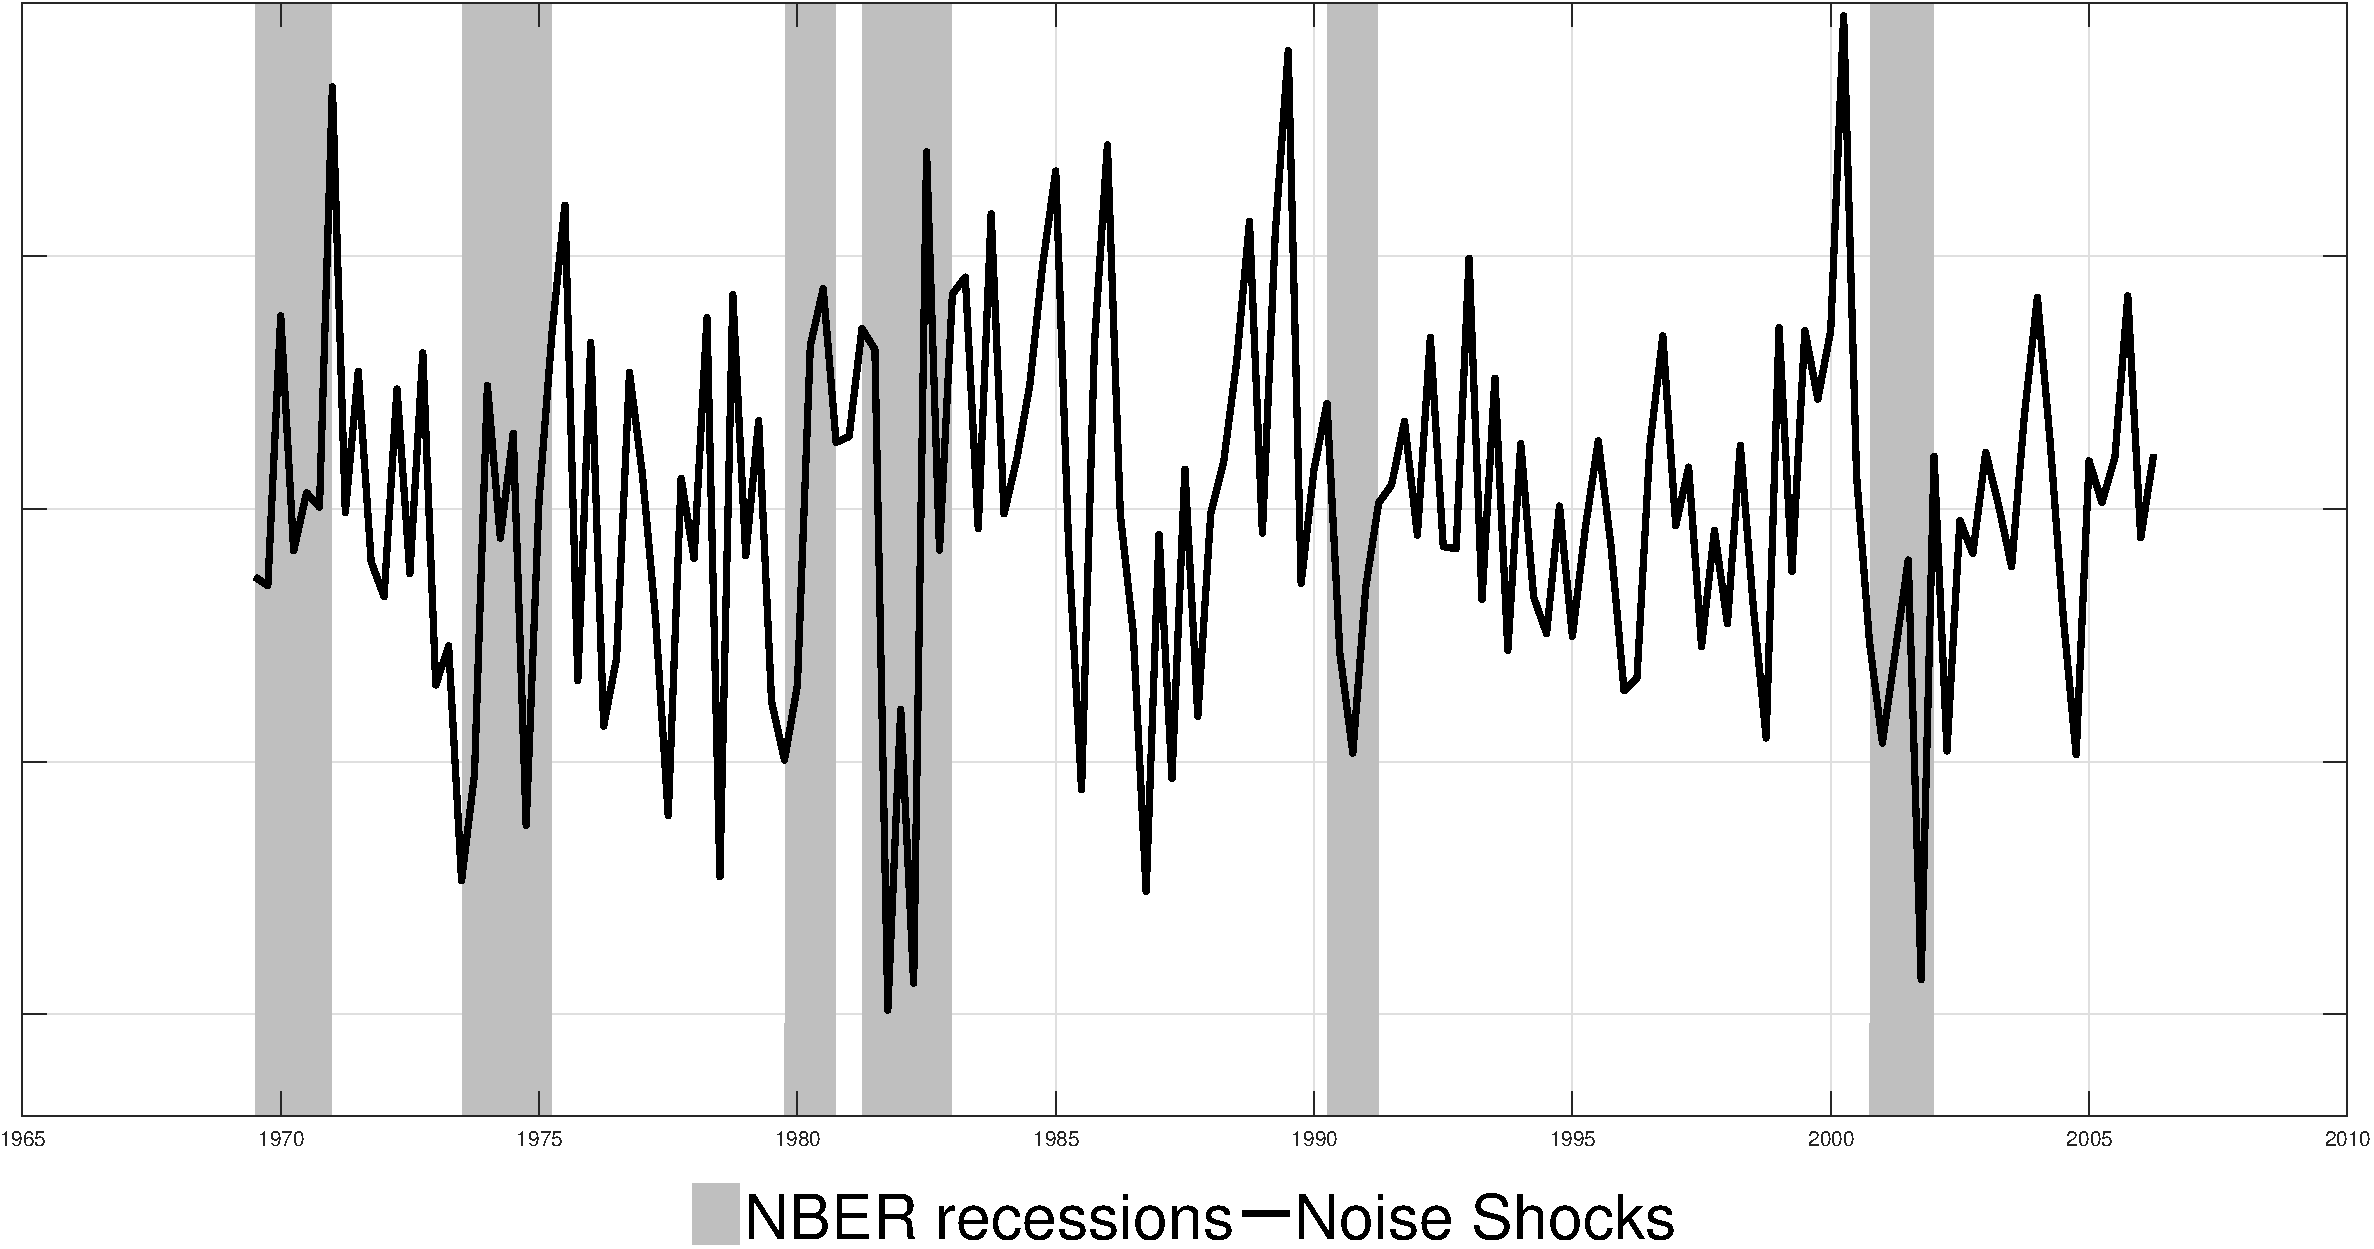
\includegraphics[scale = 0.27]{\ourFigPath Figures/Noise_Shocks_SPF_GDPgrowth_revisions}
\end{center}

}


\frame{\frametitle{Step 2 - Estimation of IRFs to $\tilde{Z}_t$}
	Define $Y_t$ to be the log-transformation of an endogenous aggregate macroeconomic variable.
	
	\
	
	Using standard OLS techniques we estimate $H$ regressions	
	$$
	Y_{t+h} = C + \gamma T_t + \Theta_h^Y \tilde{Z}_t + \delta X_{t-1} + \epsilon_{t+h}
	$$
	where
	\begin{itemize}
		\item $h = 1,2, \dots, H$ represent the forecast horizon
		\item $C$ is a constant parameter
		\item $T_t$ is a linear time trend
		\item $X_t$ is a vector of control variables at $t-1$: TFP, PC, ...
	\end{itemize}
	
	\
	
$\Theta_1^Y, \ \Theta_2^Y, \ \dots, \ \Theta_H^Y$ represent the path of the impulse response function of $Y_t$ to a unit deviation of $\tilde{Z}_t$.
	
}

\frame{\frametitle{Bootstrapping Techniques}
	
	\begin{enumerate}
		 

	
\item Consider the tuple $\Gamma^Y_h = \{ Y_{t+h}, \ T_t, \ \tilde{Z}_t, \ X_{t-1} \}$.

\

\item Divide $\Gamma^Y_h$ over time $t$ in smaller blocks and randomly reorder these blocks in order to form a new tuple $\Gamma^Y_{h,Boot1}$ of the same size of the previous one.

\


\item Estimate $\Theta_{h,Boot1}$ from $\Gamma^Y_{h,Boot1}$ using standards OLS techniques.

\

\item Redo (1)-(3) $2000$ times and select confidence intervals.

	\end{enumerate}	
	
}

\frame{\frametitle{Local Projection - Confidence Interval 68\% and 90\%}
	
	\begin{center}
		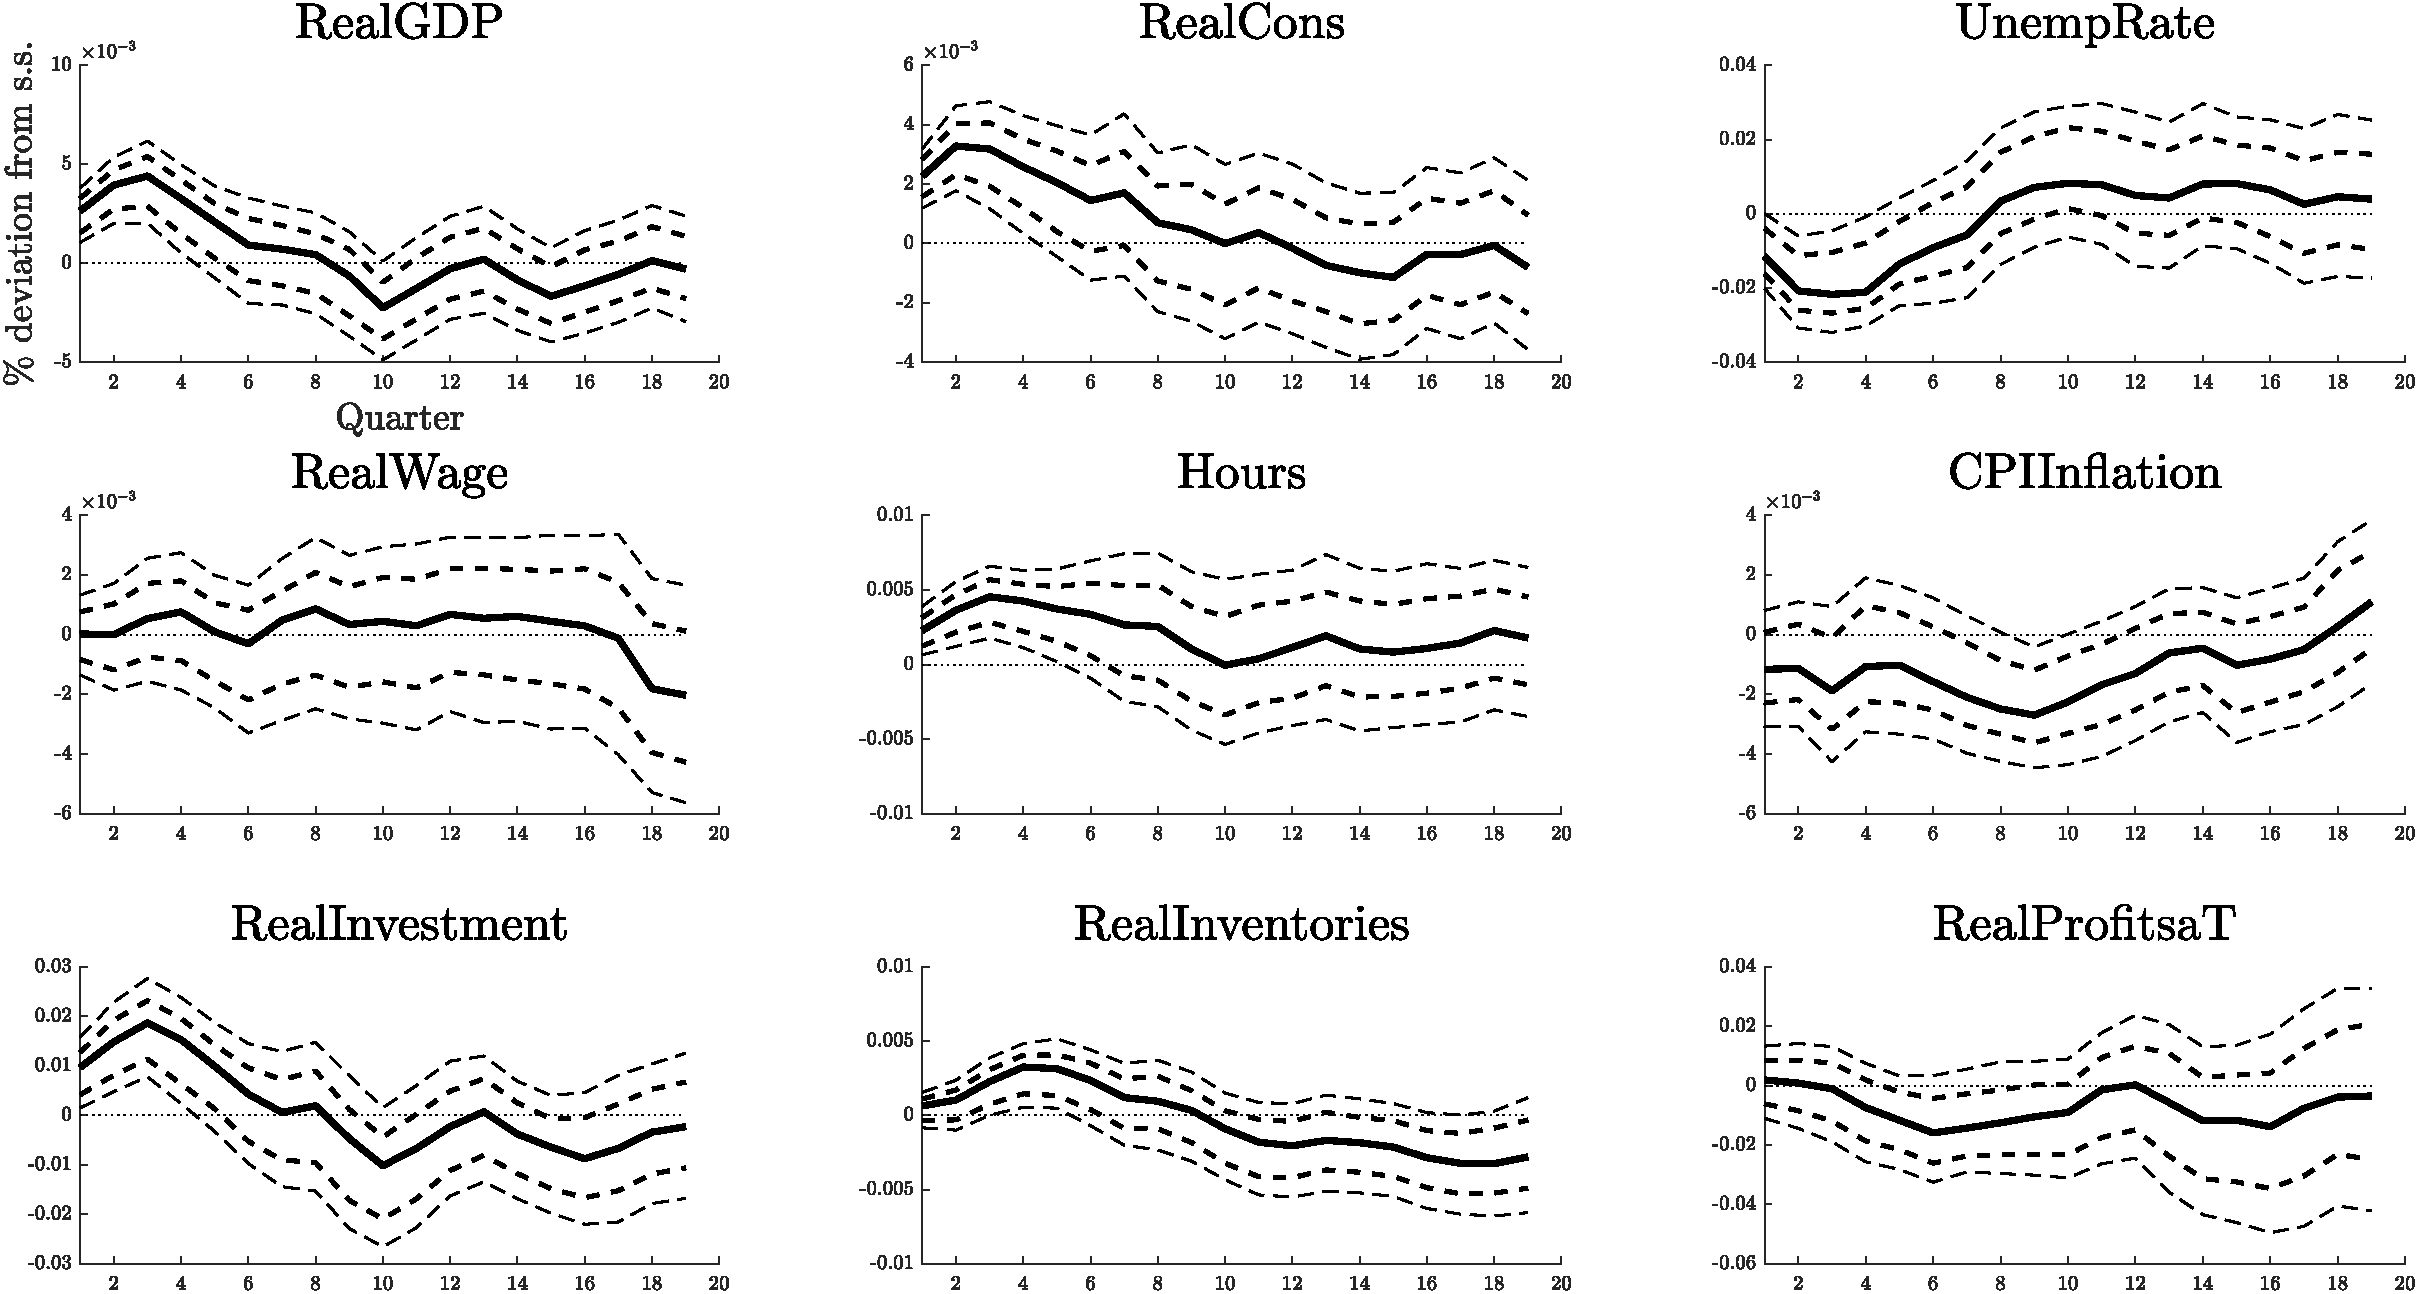
\includegraphics[scale = 0.27]{\ourFigPath Figures/Unconditional_RyanPresentation_8_28_2018_loglevels}
	\end{center}
	
	
}

\frame{\frametitle{Robustness Check}
	
	\begin{center}
		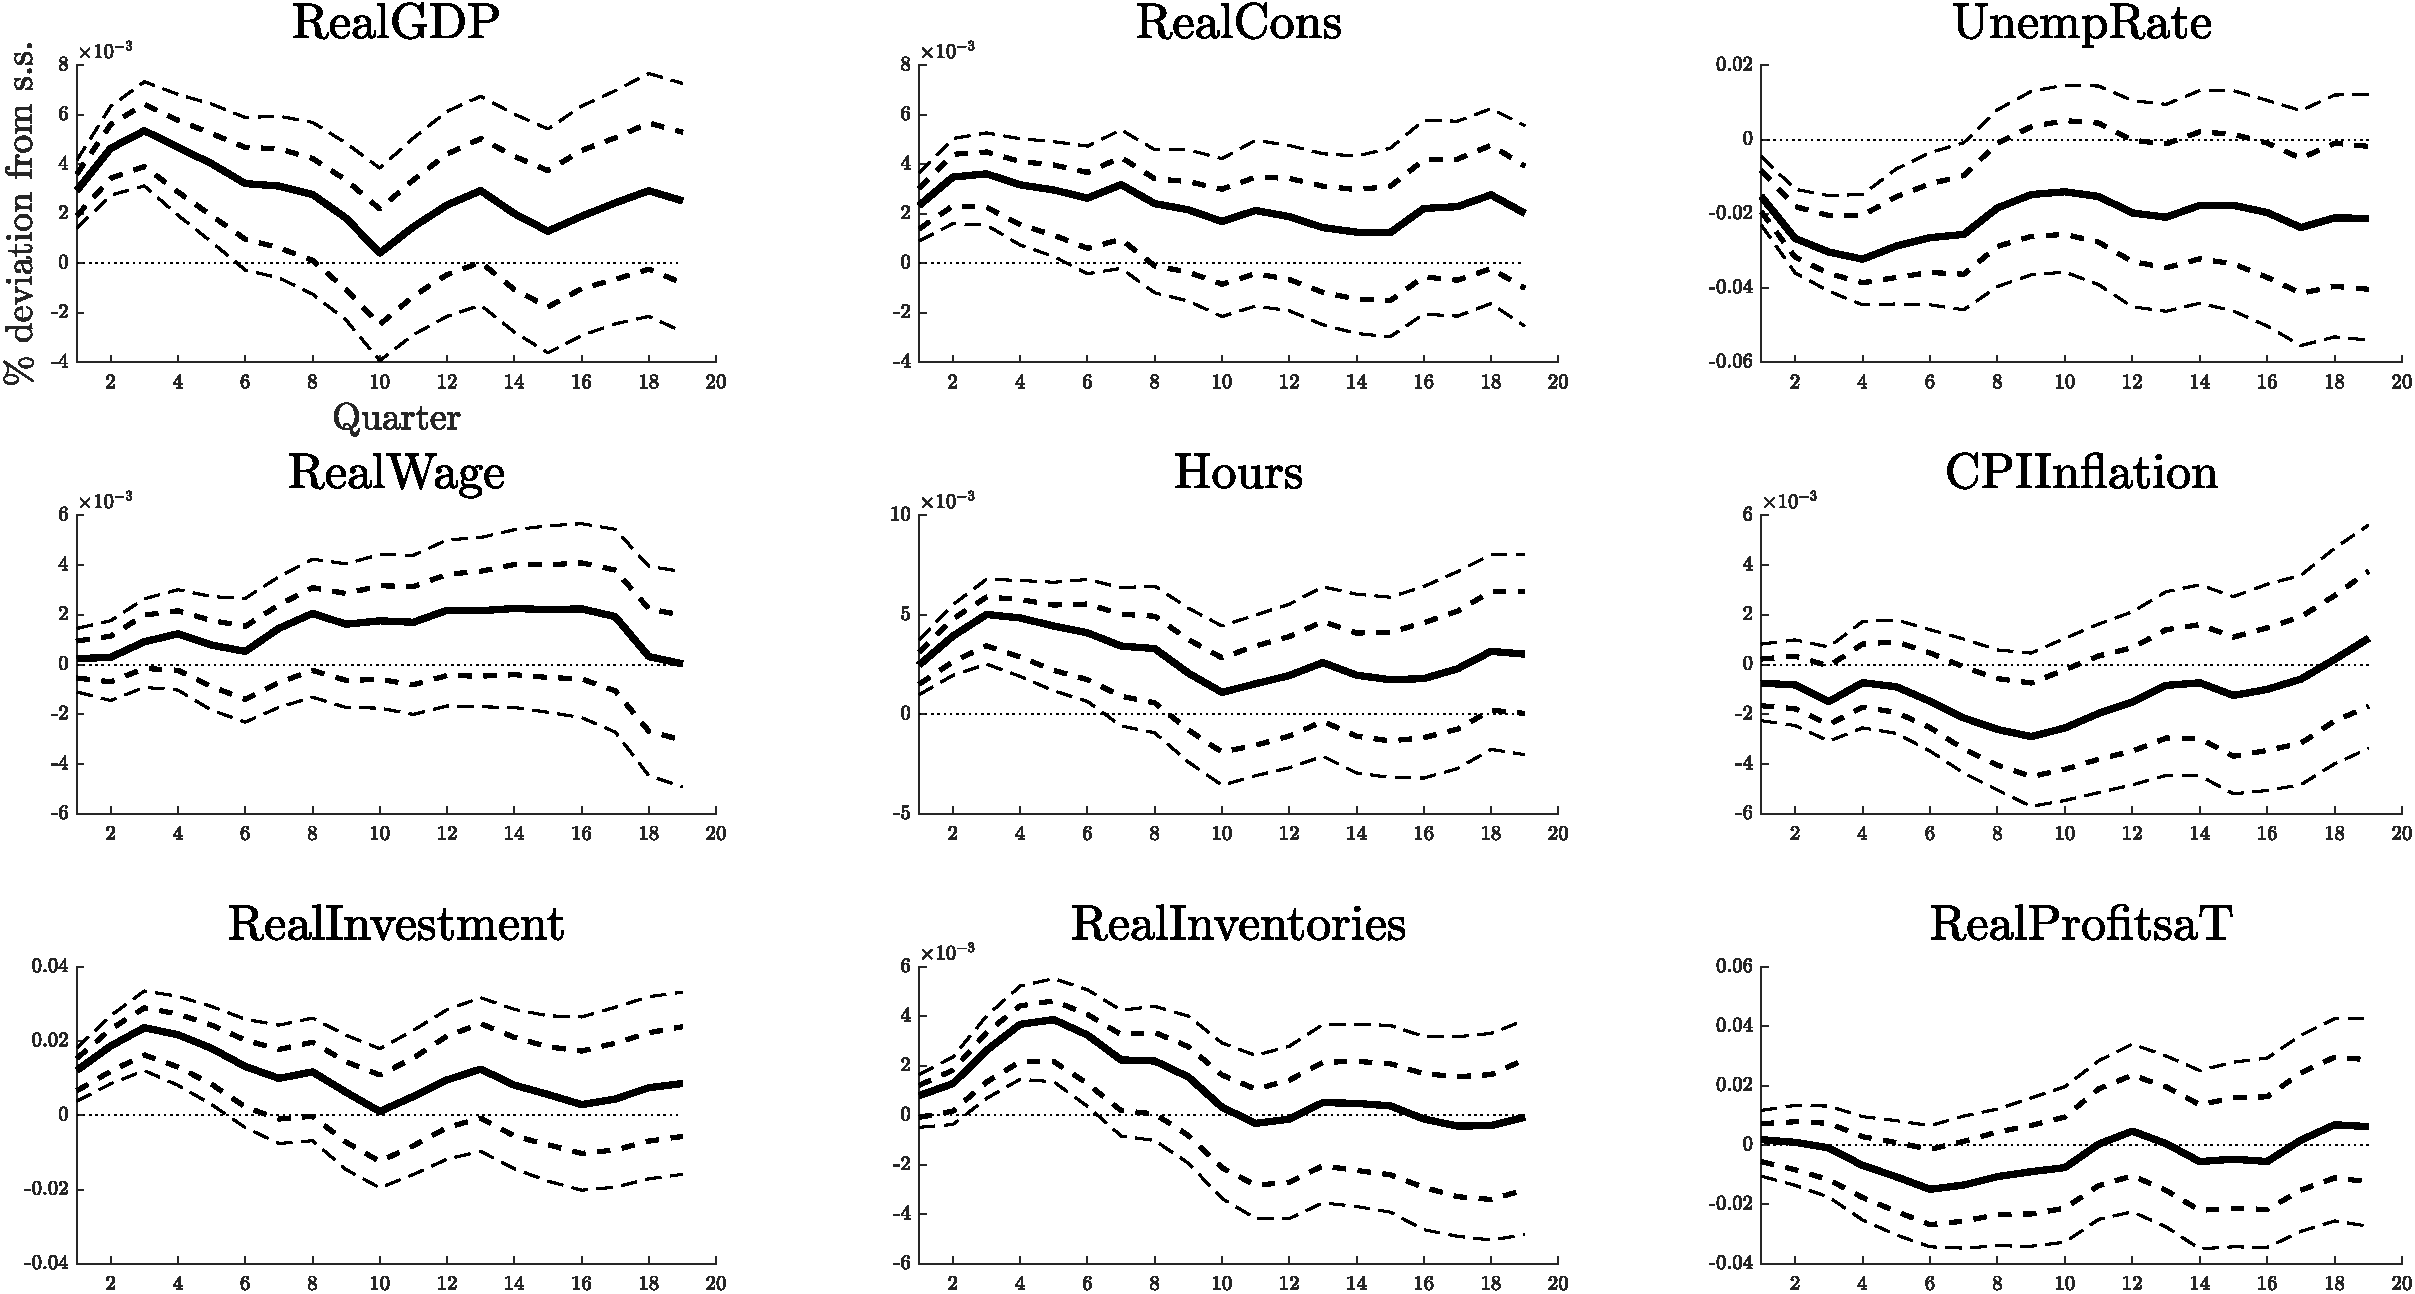
\includegraphics[scale = 0.27]{\ourFigPath Figures/Unconditional_RyanPresentation_8_28_2018_logdifferences}
	\end{center}
		
}












\end{document}